% !TEX root = ../thesis-example.tex
%
\chapter{Architecture of Chrysalis}
\label{sec:init}

Since \emph{Chrysalis} was handed to us as an already running prototype including a predefined layer structure and a way to interact with it in a browser, those designs were therefore a given. The Application is written entirely in JavaScript code, with the code deployed to the Blockchains being an exception sometimes.
The prototype version was able to run on an \emph{Ethereum}-Blockchain-Network, demonstrating it's functionality.
In this chapter, we elaborate on the general structure of \emph{Chrysalis}, omitting technical details and focusing on how the user and the components interact.

\section{Intended Usage}
\label{sec:init:usage}

From the user's point of view, three interactions with the system are generally intended, as they're described below. The configuration aside, the other two, encapsulating BPM, are shown in figure \ref{fig:init:usage:bpm}.

\begin{figure}[h]
	\centering
	\captionsetup{justification=centering,margin=2cm}
	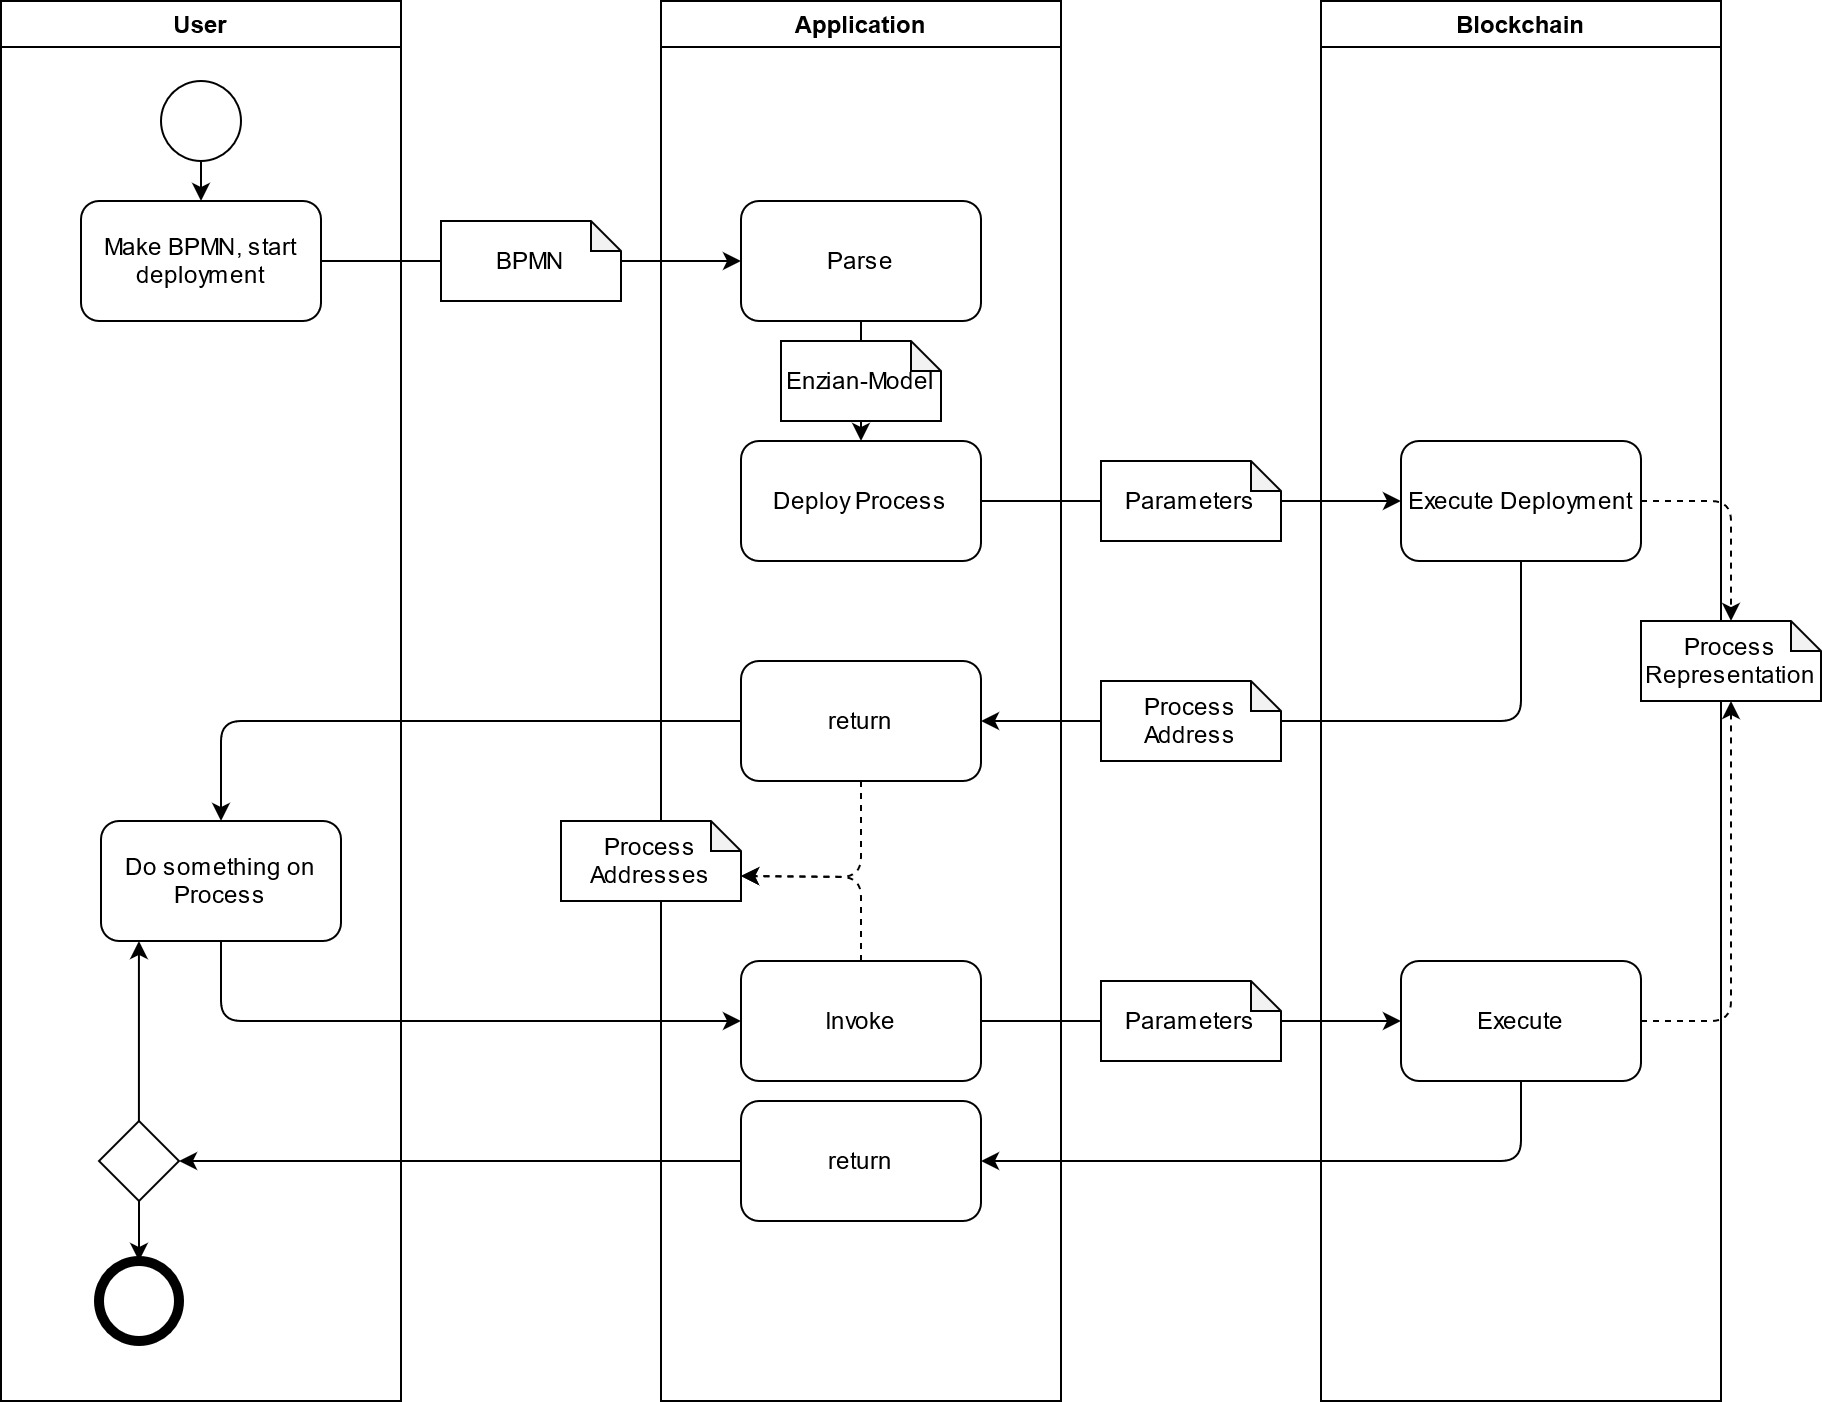
\includegraphics[height=0.7\textwidth]{gfx/bpmn2bc}
	\caption{Layer structure of the original \emph{Chrysalis} System.}
	\label{fig:init:usage:bpm}
\end{figure}

\textbf{Configuration} \\[0.2em]
TODO config

\textbf{Process Deployment} \\[0.2em]
TODO deployment

\textbf{Process Execution} \\[0.2em]
TODO execution

\section{Components and their Interactions}
\label{sec:init:components}


\begin{figure}[h]
	\centering
	\captionsetup{justification=centering,margin=2cm}
	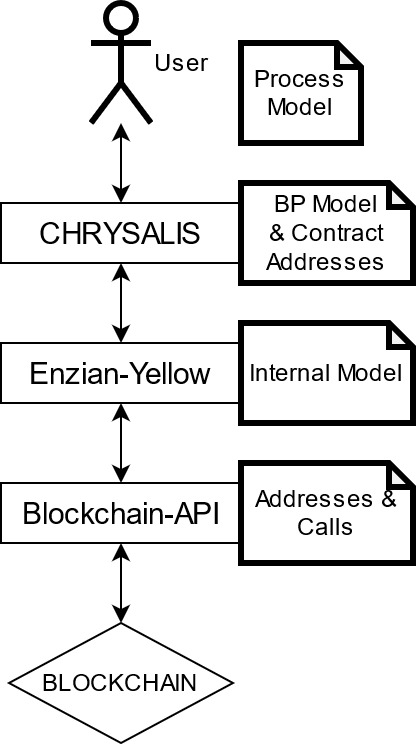
\includegraphics[height=0.5\textwidth]{gfx/init-components-layers}
	\caption{Layer structure of the original \emph{Chrysalis} System.}
	\label{fig:init:components:layers}
\end{figure}

The name-giving component, \emph{Chrysalis}, is a front-end application written in \emph{React} (for disambiguation, we will refer to the component as 'Chrysalis' and the entire system as 'project'). While it serves as a window for the user to interact with, it also handles the storage of any relevant data, like the addresses of deployed processes and authentication credentials of the user. \emph{Chrysalis}, like any React-app, deploys a packaged version of itself and it's dependencies into the user's browser, to be executed there. As for business process interactions, it instantiates an \emph{Enzian-Yellow} object with the fitting configuration and delegates all commands to it.

\emph{Enzian-Yellow}, being an installed dependency of \emph{Chrysalis}, does the abstraction work between BPM actions and Blockchain operations. When instantiated and configured, it will in turn instantiate and configure a Blockchain-API to connect to the corresponding network node. \emph{Enzian-Yellow} offers methods like creating and deploying processes and executing tasks, which are internally translated into the corresponding API invocations, and vice versa for the node's responses.

The \emph{Blockchain-API} is the gateway from a local program to interact with a specified Blockchain network node. When instantiated, it establishes a connection to the specified node, handles authorization work and abstracts the networking away, so that the Blockchain's data and functions may be used as if they were local to the code.

The \emph{Blockchain Network Node}, depicted in figure \ref{fig:init:components:layers} as 'Blockchain', usually acts like a server that has a local copy of the Blockchain. It is fully synchronous with the network and any operation on the chain (i.e., addition of blocks) will be mirrored on every node in the network. In our case this means that every BPM action will be synchronized for every network participant that way.

\section{Modeling of Processes}
\label{sec:init:model}

TODO Introduce Smart Contracts and Data as primary Blockchain Components
TODO explain how Processes are represented with those.

